% !TEX root = ../thesis.tex

\chapter{Modelling motion on the \tsc{ER}}\label{sec:modelling}

The messy behaviour of Aβ molecules we saw in \cref{sec:data_analysis} by the analysis of \tsc{SPT} data suggests a new hypothesis. The complex and delocalised dynamics that we found may involve active transport on the \emph{endoplasmic reticulum}, a network like organelle supporting various functions encompassing protein folding and redistribution. While it is known that the \tsc{ER} is acts as an active transportation network, it is not possible to find a directionality and the dynamics of such transport mechanism remains not clear \cit{nehls2000dynamics}.
In a recent work, Holcman's team\cit{holcman2018single} has shown that particles moving on the \tsc{ER} follow a two-state process, characterised by alternation of a high-velocity directed motion state associated to flow in the network tubules and a low-velocity diffusing state associated to the nodes. This kind of behaviour, with particles jumping between areas of slow motion, resembles the results the analysis performed in \cref{sec:full_picture}, motivating the hypothesis that transport of Aβ is linked to the \tsc{ER}.

As the inner workings of the \tsc{ER} are not known, it would be difficult to directly compare the the results of \cref{sec:data_analysis} to the \tsc{ER} dynamics. How are molecules redistributed in the \textsc{er}? Which timescale characterise this transport process? First, we have to understand how this network works. Thus, in this chapter we will focus on a model of motion on the \tsc{ER}, building on the results of previous analysis, \cit{holcman2018single} and presenting results of numerical simulations.



\section{Active network model}

The \textsc{er} is a wide network like organelle that  spans from the nuclear envelope to the cell periphery. It has a fundamental role in the production, maturation and trafficking of proteins and lipids. A recent study based on super resolution imaging \cite{ls_er} has revealed in its entirety the \textsc{er} network structure, made amost exclusively of tubules at varying densities.

\begin{figure}
  \sidecaption{The endoplasmic reticulum of a \tsc{HEK 293T} cell imaged by fast SIM.}\label{fig:er}
  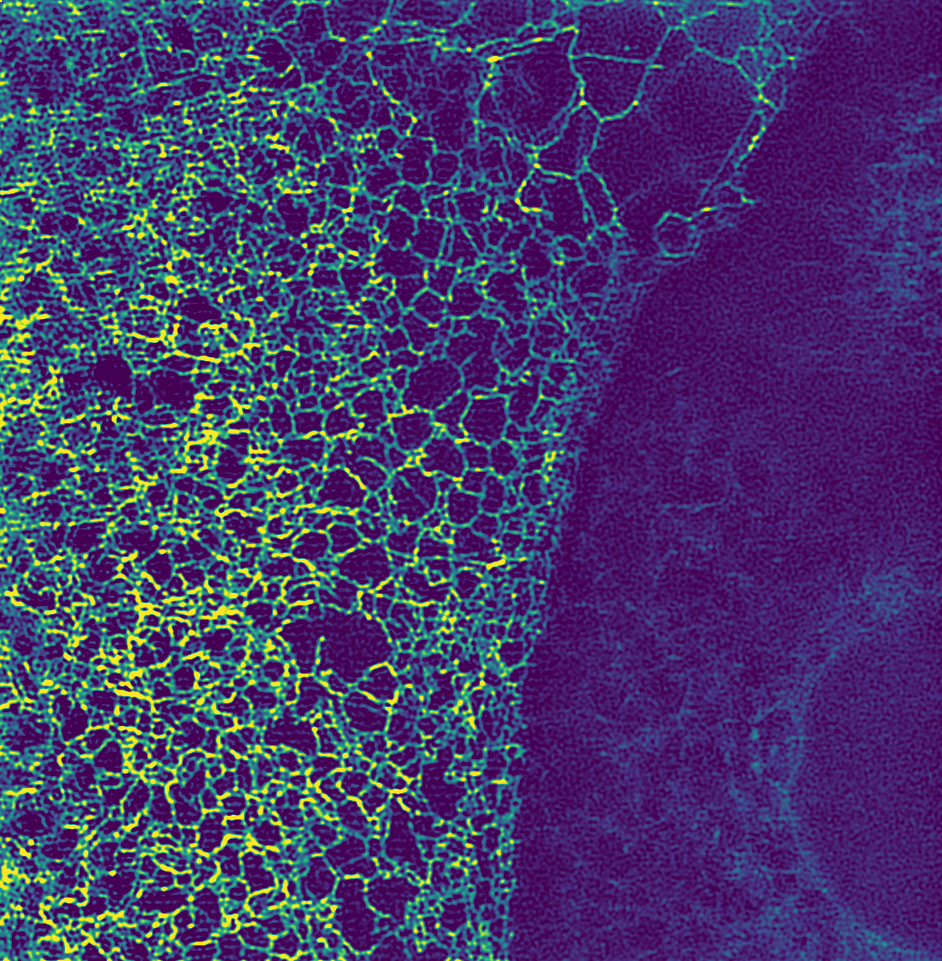
\includegraphics[width=\textwidth]{er.png}
\end{figure}


\section{Numerical simulations}
